\documentclass[12pt, a4paper]{article}
\usepackage[tmargin=2.5cm, bmargin=2.5cm, lmargin=2cm, rmargin=2cm]{geometry}
\usepackage[utf8]{inputenc}\DeclareUnicodeCharacter{2212}{-}
\usepackage[T1]{fontenc}
\usepackage{float}
\usepackage{lmodern}
\usepackage{hyperref}
\hypersetup{
colorlinks = true,
linkcolor  = NavyBlue,
citecolor = NavyBlue,
urlcolor = NavyBlue
}
% Bib stuff
\usepackage[
    backend=biber,
    style=apa,
]{biblatex}
\setlength{\bibhang}{0pt}
\setlength{\bibitemsep}{6pt}
\addbibresource[]{../peak_water.bib}
\usepackage{amsmath}
\usepackage{amssymb}
\usepackage{gensymb}
\usepackage{upgreek}
\usepackage{enumitem}
\usepackage{graphicx}
\usepackage{subcaption}
\graphicspath{{../plots/}}
\usepackage[dvipsnames]{xcolor, colortbl}
% Setup for the captions
\usepackage[hypcap=true, labelfont=bf]{caption}
\captionsetup{belowskip=2pt, aboveskip=2pt}

\author{Erik Holmgren \\ Advisor: Fabien Maussion, PhD}
\title{Master thesis proposal: Peak water using the Open Global Glacier Model}
\date{March 2021}
\begin{document}
\maketitle
\noindent
\section{Motivation}
Glacier mass loss has increased during the second half of the 20th century
\parencite{vaughanObservationsCryosphere2013} and is predicted, in all current
climate projections, to continue throughout the 21st century
\parencite{ipccClimateChange20142014}. The magnitude of the end of century
glacial mass loss varies greatly depending on the climate scenario and the
region -- \textcite{hussNewModelGlobal2015} found global glacier volumes to
decrease between 25\% (RCP2.6) and 48\% (RCP8.5) and regional losses varying
between 20 and 90\%.

% Simulating global glaciers \textcite{hussNewModelGlobal2015} found that the
% global glacier volume will decrease with 25$\pm$5\% for RCP2.6, 33$\pm$8\% for
% RCP4.5 and 48$\pm$9\% by the end of the century. Furthermore, they found large
% regional differences -- glaciers in central Europe and in low latitudes may lose
% as much as 90\% of their mass while glaciers in Arctic Canada and
% Antarctica/Subantarcitca lose 20\%. 

% End of century glacier mass exhibit a substantial spread depending on the GCM
% used for the emission scenario in the simulation. For instance, mass losses in
% Svalbard varies between 12\% and 90\% for RCP4.5
% \parencite{hussNewModelGlobal2015}.


Glaciers play an important role as a form of water storage. By capturing and
holding precipitation as snow and ice until it is released later in the ablation
season as meltwater, up to 79\% of the total annual precipitation falling onto
the glacier surface can be delayed. Regions that benefits from this delay are
particularly those that experience a warm and dry ablation season
\parencite{kaserContributionPotentialGlaciers2010}. One of those areas is the
Indus basin, where during the pre-monsoon season up to 60\% of the total
irrigation volume comes from either snow or glacier melt, resulting in an 11\%
increase of the total crop production
\parencite{biemansImportanceSnowGlacier2019}. Simultaneously, the Indus basin is
one example of a large river basin which, under the present climate, experiences
water scarcity, threatening the food security of millions of people
\parencite{kummuClimatedrivenInterannualVariability2014}. This in an area where
large amounts of the freshwater resource is shared across state borders where
the risk for armed conflict is high
\parencite{schleussnerArmedconflictRisksEnhanced2016,
pritchardAsiaShrinkingGlaciers2019}, amplifying the consequences of water
shortages. 

\textcite{mishraDifferentialImpactClimate2020} found that during the
period leading up to peak water, hydroelectric production from two basins in the
Karakoram and Central Himalayan regions would benefit from increased flows.
However, for the basin located in the Karakoram, post peak water benefits were
highly variable, an indication of high spatial variations in the impacts of
changes in glacial drainage.

The populated areas on the dry, western, slopes of the Andes are other examples
of regions depending on glacier meltwater for potable water and power
generation. \textcite{vergaraEconomicImpactsRapid2007} estimate the cost of
mitigation and adaption to retreating glaciers in the Andes to between US\$300
million and US\$1.5 billion.

\textcite{brunnerPresentFutureWater2019} found that basins in Switzerland
experience water shortage during the summer months in runoff simulations based
on future climate scenarios. Shortages were elevated in basins highly dependent
on runoff from ice and snow melt. However, the model used (PREVAH, see
\cite{viviroliIntroductionHydrologicalModelling2009}) does not handle glacier
evolution i.e. mass changes, and for this reason it is likely overestimating the
future contribution of glacial runoff to the seasonal water supply. 3 to 4\% of
the total annual energy production from hydropower in Switzerland currently
originates from glacier mass loss, a finite resource that is expected to decline
over the coming decades \parencite{schaefliRoleGlacierRetreat2019}. 

% of glacier melt include significant contributions to sea level rise (e.g.
% \cite{marzeionFutureSealevelChange2012a})

% More direct societal impacts The Indus basin is experiencing water scarcity under the present climate
% \parencite{kummuClimatedrivenInterannualVariability2014}.

% Out of the total precipitation falling onto the glacier surface, between 79 and
% 17\% will experience a seasonal delay -- meaning that the water will be stored
% in the glacier and released later in the season. The relative importance of
% glacier melt water to the basin water availability decreases in the presence of
% liquid precipitation, hence the positive effects of seasonally delayed water
% release from glaciers are more pronounced in areas experiencing warm and dry
% ablation seasons \parencite{kaserContributionPotentialGlaciers2010}.

% The monthly percentage of total water input to a basin that experience seasonal
% delayed water release by glaciers decreases downstream the river while the
% population generally increases. Thus, the societal impacts of seasonal delayed
% water release by glacier melt reaches a maximum at intermediate altitude bands
% \parencite{kaserContributionPotentialGlaciers2010}.

\section{State of the art -- Glacial hydrology}
Glaciers store water in multiple ways -- as a liquid in surface snow and firn,
in crevasses, drainage networks, englacial pockets and surface pools, or as a
solid in the form of snow, firn and ice
\parencite{janssonConceptGlacierStorage2003}. The main factors controlling the
discharge hydrograph of an alpine basin are the topographical structure, the
seasonal air temperature gradient, the seasonal distribution of precipitation
\parencite{zappaSeasonalWaterBalance2003}, and the size of the glaciated area
within the basin \parencite{janssonConceptGlacierStorage2003}. 

Melt is the largest contributor to glacier runoff, hence the fraction of summer
runoff to the annual runoff increases with an increased glaciation in a basin
\parencite{zappaSeasonalWaterBalance2003,chenInfluenceAlpineGlaciers1990}.
\textcite{blissGlobalResponseGlacier2014} showed that glacier net
mass loss is an important part of the total glacier runoff, indicating that the
societal importance of glacier melt water might be higher than the estimates
from \textcite{kaserContributionPotentialGlaciers2010}, where runoff estimates
were done under an assumed equilibrium and thus neglecting any runoff resulting
from net mass loss.
% Glacier runoff peaks late in the summer -- when the melt line has crept further
% up and thus exposing more of the catchment area to melt
% \parencite{zappaSeasonalWaterBalance2003}.

% In alpine catchments snow accumulation and snow melt are the main contributors
% to runoff generation, while the influence of precipitation is small, during the
% months between June and October \parencite{zappaSeasonalWaterBalance2003}. 

% The estimated the societal importance of glacier melt water from
% \textcite{kaserContributionPotentialGlaciers2010} was made under the assumption
% that the glaciers were in equilibrium with the local climate -- i.e. none of the
% runoff estimations included any net mass loss.

The term \emph{peak water} is an adaption of the more well known term \emph{peak
oil} -- which indicates the period in time when production of oil reaches a
maximum, after which it begin to decrease \parencite{gleickPeakWaterLimits2010}.
Recently this term has been applied to meltwater generation from glaciers (e.g.
\cite{hussGlobalscaleHydrologicalResponse2018}) as a way to put the impacts of
shrinking glaciers into a societal context. The mechanism behind glacial peak
water is as follows (see Fig. \ref{fig:peak_water}): When climate change causes
a glacier to recede, water is released from long term glacial storage. The
annual runoff will increase until a maximum, i.e. peak water, is reached. At
this point and forward the annual runoff will begin to decrease, since the area
of the shrinking glacier is no longer able to produce the same amounts of
meltwater \parencite{janssonConceptGlacierStorage2003}. If the glacier reaches a
new state of equilibrium (zero net mass loss), the annual runoff from the
initially glaciated area might return to pre-peak water levels. However, runoff
levels during the melt season can be expected to fall below the pre peak water
levels since melt water originating from long term storage will be reduced
\parencite{hussGlobalscaleHydrologicalResponse2018,
ragettliContrastingClimateChange2016, immerzeelRisingRiverFlows2013}.
\begin{figure}[h]
    \centering
    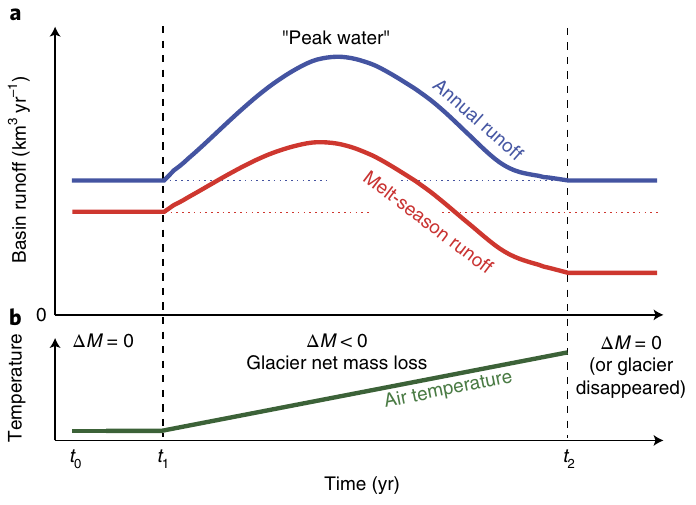
\includegraphics[width=0.6\textwidth]{../peak_water.png}
    \caption{Schematised view of glacier runoff and peak water during a
    transient state. The annual glacier runoff will be constant from year to
    year during equilibrium. If the conditions change so that the glacier is no
    longer in equilibrium with its climate and the glacier begins to lose mass,
    the melt season runoff will increase with rising temperatures.
    Adapted from \textcite{hussGlobalscaleHydrologicalResponse2018}.}
    \label{fig:peak_water}
\end{figure}

\section{Peak water using the Open Global Glacier Model}
State of the art peak water estimations (e.g.
\cite{rounceGlacierMassChange2020,hussGlobalscaleHydrologicalResponse2018}) have
relied on parametrizing the re-distribution of mass throughout the glacier with
so called mass re-distribution curves, developed by
\textcite{hussFutureHighmountainHydrology2010}. This parameterization is a clear
step up in performance compared to previous ice flow parametrizations (e.g.
length-area scaling), but still relies on multiple digital elevation models
covering the glacier for calibration of the flow as a function of the mass
balance. As a consequence, the flow, or mass re-distribution, of non-measured
glaciers is estimated from known glaciers of a similar size, without
considering topographical differences. 

The common approach for calculating glacial runoff is to imagine a so called
fixed gauge station -- a hypothetical measuring station at the terminus of the
glacier, measuring all water leaving the initially glaciated area. Runoff, $Q$,
is calculated from the ablation $\alpha$, the liquid precipitation $p_{liquid}$,
and the refreezing of meltwater within the glacier $R$ as
\begin{equation}
    Q = \alpha + p_{\mathrm{liquid}} - R.
\end{equation}
The contribution from ablation is made up of ice and snow melt, also known as
the excess melt water from the glacier. The total excess meltwater is equivalent
to the total mass loss over a period of time. It is produced during years with
negative mass balances, but since the mass balance can vary from year to year,
excess meltwater is only produced from committed mass loss. Because of this, in
order to maintain the total, excess meltwater has to be calculated retroactively
for each mass-balance year. This process starts with calculating the total
excess meltwater for the selected time period, e.g. net mass change at 2100. The
total excess meltwater can then be distributed, sequentially, to all negative
mass-balance years where mass is not regained in the future. This way the total
excess melt water is maintained, even if the cumulative sum of negative mass
balance years exceeds the net mass change
\parencite{rounceGlacierMassChange2020}. Runoff originating from liquid
precipitation is measured from the initially glaciated area. As the glacier
shrinks, this part of the runoff is divided into two parts: on-glacier runoff
and off-glacier runoff. Other processes, such as evapotranspiration or
ground-water recharge, are considered negligible and are not included in glacier
runoff calculations.

Employing the Open Global Glacier Model (OGGM,
\cite{maussionOpenGlobalGlacier2019}) for peak water calculations would be the
first time a physical ice flow model is applied globally to calculate glacier
runoff. It would be a step towards mitigating the problem of
over-parametrization present in the current global glacier models used for
hydrological analysis. Including ice dynamics in global glacier simulations
results in reduced ice losses compared to parametrized models
\parencite{zekollariModellingFutureEvolution2019}, possibly leading to more
accurate runoff estimations. The inclusion of ice dynamics also enables the
glacier to grow, if climatic conditions allow it, and not only to shrink, a
limitation of mass re-distribution curves. Simulating peak water with the OGGM
will provide a new view of global glacier runoff and peak water estimations with
fewer parametrizations. This approach will build on the previous peak water
research and provide valuable information on future water availability in
glaciated areas. 

% A new set of runoff estimates, based on a different modelling framework, will
% broaden the scientific background about the subject. The OGGM uses the same
% mass balance scheme, a degree day model, as for example PyGEM (used by
% \cite{rounceGlacierMassChange2020}). Thus, any differences in the annual mass
% balance should stem from the different implementations of ice dynamics --
% possibly leading to slightly different area/length estimations and thus a
% different runoff.


\subsection{Research questions}
For this thesis I will work towards answering the following questions:
\begin{enumerate}
    \item \textbf{How does the inclusion of ice dynamics in a global glacier
    model change the temporal and spatial variation of peak water?} The
    inclusion of ice dynamics will result in a different annual mass balance
    compared to models relying on parametrizing the mass re-distribution.
    Because of this, the projected timing of peak water can be expected to
    change.
    \item \textbf{When will the basins most dependent on glacier runoff reach
    peak water?} The Indus basin lies in a region where glacial storage and the
    subsequent seasonal delay of runoff is particularly important for
    agriculture. Future changes to the runoff patterns would require adaption to
    maintain water availability during the dry pre-monsoon season. An accurate
    estimation of peak water would provide a time frame for this adaption. This
    would corroborate on the studies done on High Mountain Asia by
    \textcite{rounceGlacierMassChange2020} and
    \textcite{hussGlobalscaleHydrologicalResponse2018}.
    \item \textbf{At what levels, and during which time, will runoff levels
    begin to stabilise?} Peak water gives a measure of when the annual runoff
    from glaciers reaches a maximum, but concerning societal impacts the long
    term, stabilised levels, are more interesting. With seasonal weather
    patterns likely becoming more extreme in Europe, e.g. more frequent heat
    waves and droughts \parencite{ipccClimateChange20142014a}, good estimates of
    future runoff levels in glaciated areas are essential for climate change
    adaption and planning. This include an analysis of the seasonal hydrograph,
    the annual runoff of a basin might return to pre-peak water levels, but
    meltwater during the summer months might be reduced.

    % \item \textbf{How will the seasonal hydrograph change for future runoff
    % projections?} When will the seasonal discharge occur under future scenarios
    % and how might it affect the beneficial impacts of glacial water storage.
    % \item \textbf{Societal impacts???} There seems to be a gap in the knowledge
    % about societal importance of glacier runoff with regards to glacier mass
    % evolution. Impact estimates are not considering the possible runoff decline
    % in some regions.
\end{enumerate}

Hydrological outputs were recently implemented in the OGGM, but still need to be
evaluated and fully integrated into the model. The first step of this work is to
make sure that runoff calculations in the OGGM are working as intended. This
include testing the implementation, running a few simulations on a smaller scale
and document it. In the current state OGGM outputs hydrological measurements on
an annual scale. However, monthly outputs will be added, enabling the analysis
of seasonal runoff.

Based on the results from previous studies, a number of regions interesting in
regards to peak water can be selected for simulations using the OGGM. To
evaluate the affect of including ice dynamics in glacier runoff simulations, the
results will be compared to previous studies (e.g.
\cite{rounceGlacierMassChange2020,hussGlobalscaleHydrologicalResponse2018}). The projected runoff estimates of European basins can be compared to current
levels in order to assess the future impact of diminishing glacier melt.

\printbibliography
\end{document}